\chapter{Peruuttava haku}

\index{backtracking}
\emph{Peruuttava haku} (\emph{backtracking}) on menetelmä,
jossa on ideana käydä läpi kaikki mahdolliset tavat 
ratkaista annettu tehtävä.
Peruuttava haku on luontevaa toteuttaa rekursion avulla,
jolloin jokainen rekursion haara vastaa yhtä tapaa
viedä ratkaisua eteenpäin.

\emph{Peruuttava haku} (\emph{backtracking}) on menetelmä,
jossa on ideana käydä läpi kaikki mahdolliset tavat 
ratkaista annettu tehtävä.
Peruuttava haku on luontevaa toteuttaa rekursion avulla,
jolloin jokainen rekursion haara vastaa yhtä tapaa
viedä ratkaisua eteenpäin.

\section{Silmukoista rekursioon}

Aloitamme peruuttavaan hakuun tutustumisen tehtävästä,
jossa haluamme muodostaa kaikki yhdistelmät,
joissa on peräkkäin $n$ kokonaislukua väliltä $1 \dots m$.
Tällaisia yhdistelmiä on kaikkiaan $m^n$,
koska joka kohdassa on $m$ tapaa valita luku.
Esimerkiksi jos $n=3$ ja $m=4$, mahdollisia yhdistelmiä
ovat esimerkiksi $[1,2,1]$ ja $[3,1,4]$
ja yhdistelmiä on yhteensä $4^3=64$.

Luonteva tapa ratkaista tehtävä tietylle $n$:n arvolle on
luoda $n$ sisäkkäistä silmukkaa, joista jokainen käy $m$ lukua läpi.
Esimerkiksi seuraava koodi käy läpi kaikki yhdistelmät
tapauksessa $n=3$ ja $m=4$:

\begin{code}
for a = 1 to m
    for b = 1 to m
        for c = 1 to m
            print(a,b,c)
\end{code}

Tämä on sinänsä mainio ratkaisu, mutta siinä on yksi ongelma:
lukujen määrä $n$ vaikuttaa silmukoiden määrään.
Jos haluaisimme muuttaa $n$:n arvoa, meidän täytyisi muuttaa
koodin silmukoiden määrää, mikä ei ole hyvä asia.
Peruuttavan haun avulla voimme kuitenkin toteuttaa ratkaisun
rekursiivisesti niin, että sama koodi toimii kaikille $n$:n arvoille.

\subsection{Haun toteutus}

Seuraava rekursiivinen proseduuri \texttt{haku} muodostaa
yhdistelmiä peruuttavan haun avulla.
Parametri $k$ tarkoittaa kohtaa, johon seuraava luku asetetaan.
Jos $k=n$, jokin yhdistelmä on valmistunut, jolloin se tulostetaan.
Muuten haku käy läpi kaikki tavat sijoittaa kohtaan $k$ luku $1 \dots m$
ja jatkaa rekursiivisesti kohtaan $k+1$.
Haku lähtee käyntiin kutsulla \texttt{haku}(0),
ja \texttt{luvut} on $n$-kokoinen taulukko, johon yhdistelmä muodostetaan.

\begin{code}
procedure haku(k)
    if k == n
        print(luvut)
    else
        for i = 1 to m
            luvut[k] = i
            haku(k+1)
\end{code}

Kuva \ref{fig:perhak} näyttää, miten peruuttava haku lähtee liikkeelle
tapauksessa $n=3$ ja $m=4$.
Merkki $-$ tarkoittaa lukua, jota ei ole vielä valittu.
Haun ensimmäinen taso valitsee yhdistelmän
ensimmäisen luvun kohtaan $0$.
Tämän valintaan on neljä vaihtoehtoa ($1 \dots 4$),
joten haku haarautuu neljään osaan valitsemaan lukua kohtaan $1$.
Jokainen haara jatkaa vastaavasti eteenpäin
ja valitsee muut yhdistelmään kuuluvat luvut.

\begin{figure}
\center
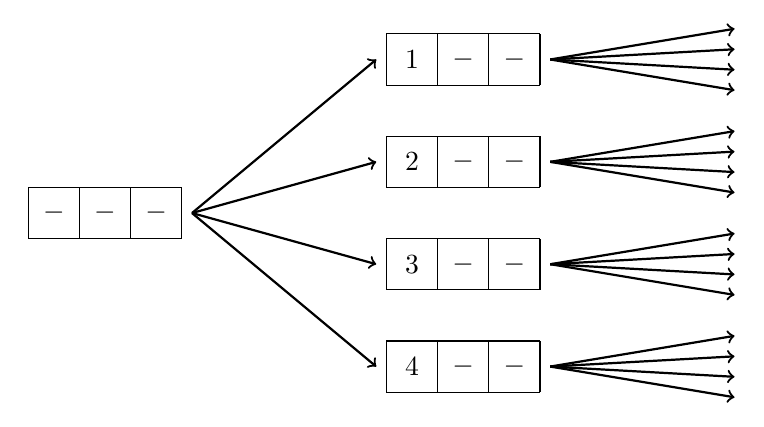
\begin{tikzpicture}[scale=.65]
    \draw (0,0) grid (3,1);
    \foreach \x/\v in {0/-,1/-,2/-} \node at (\x+0.5,0.5) {$\v$};

    \draw (7,-3) grid (10,-2);
    \foreach \x/\v in {0/1,1/-,2/-} \node at (\x+7.5,3.5) {$\v$};
    \draw (7,-1) grid (10,0);
    \foreach \x/\v in {0/2,1/-,2/-} \node at (\x+7.5,1.5) {$\v$};
    \draw (7,1) grid (10,2);
    \foreach \x/\v in {0/3,1/-,2/-} \node at (\x+7.5,-0.5) {$\v$};
    \draw (7,3) grid (10,4);
    \foreach \x/\v in {0/4,1/-,2/-} \node at (\x+7.5,-2.5) {$\v$};

    \draw[->,thick] (3.2,0.5) -- (6.8,3.5);
    \draw[->,thick] (3.2,0.5) -- (6.8,1.5);
    \draw[->,thick] (3.2,0.5) -- (6.8,-0.5);
    \draw[->,thick] (3.2,0.5) -- (6.8,-2.5);
    
    \foreach \y in {3.5,1.5,-0.5,-2.5} \foreach \z in {0.6,0.2,-0.2,-0.6}
        \draw[->,thick] (10.2,\y) -- (13.8,\y+\z);
\end{tikzpicture}
\caption{Peruuttavan haun alku tapauksessa $n=3$ ja $m=4$.}
\label{fig:perhak}
\end{figure}

Voimme arvioida algoritmin tehokkuutta laskemalla,
montako kertaa proseduuria \texttt{haku} kutsutaan yhteensä haun aikana.
Proseduuria kutsutaan kerran parametrilla $0$,
$m$ kertaa parametrilla $1$, $m^2$ kertaa parametrilla $2$, jne.,
joten kutsujen määrä on yhteensä
\[
1+m+m^2+\dots+m^n = \frac{m^{n+1}-1}{m-1} = O(m^n).
\]
Jokainen proseduurin kutsu vie aikaa $O(m)$,
koska se joko tulostaa $m$ luvun yhdistelmän tai
haarautuu rekursiivisesti $m$ osaan.
Niinpä algoritmin kokonaisaikavaativuus on $O(m^{n+1})$.

\subsection{Osajoukkojen muodostus}

\subsection{Permutaatioiden muodostus}

\section{Esimerkki: Kuningatarongelma}

Ensimmäinen tehtävämme on
laskea, monellako tavalla $n \times n$ -shakkilaudalle voidaan
sijoittaa $n$ kuningatarta niin, etteivät mitkään kaksi kuningatarta
uhkaa toisiaan. Kaksi kuningatarta voivat uhata toisiaan
pysty-, vaaka- tai vinosuuntaisesti.
Esimerkiksi tapauksessa $n=4$ mahdollisia sijoitustapoja on 2,
jotka on esitetty kuvassa \ref{fig:kuning}.


\begin{figure}
\center
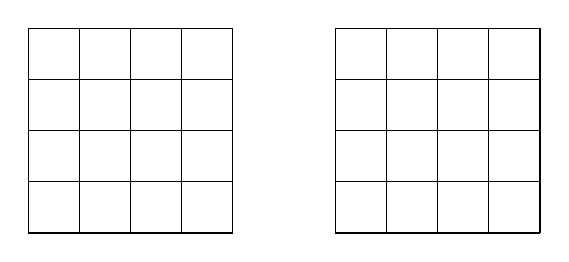
\begin{tikzpicture}[scale=.65]
  \begin{scope}
    \draw (0, 0) grid (4, 4);
    \node at (1.5,3.5) {$\symqueen$};
    \node at (3.5,2.5) {$\symqueen$};
    \node at (0.5,1.5) {$\symqueen$};
    \node at (2.5,0.5) {$\symqueen$};

    \draw (6, 0) grid (10, 4);
    \node at (6+2.5,3.5) {$\symqueen$};
    \node at (6+0.5,2.5) {$\symqueen$};
    \node at (6+3.5,1.5) {$\symqueen$};
    \node at (6+1.5,0.5) {$\symqueen$};
  \end{scope}
\end{tikzpicture}
\caption{Mahdolliset tavat asettaa 4 kuningatarta $4 \times 4$ -shakkilaudalle.}
\label{fig:kuning}
\end{figure}

\begin{figure}
\center
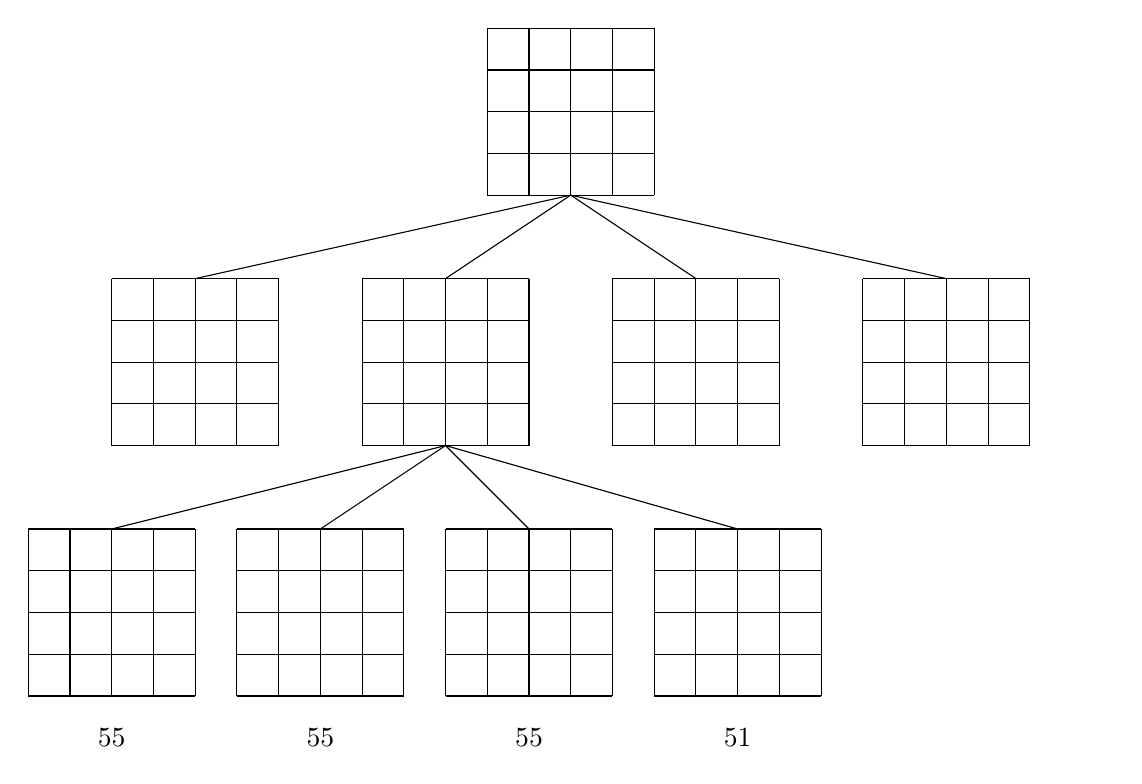
\begin{tikzpicture}[scale=.53]
  \begin{scope}
    \draw (0, 0) grid (4, 4);

    \draw (-9, -6) grid (-5, -2);
    \draw (-3, -6) grid (1, -2);
    \draw (3, -6) grid (7, -2);
    \draw (9, -6) grid (13, -2);

    \node at (-9+0.5,-3+0.5) {$\symqueen$};
    \node at (-3+1+0.5,-3+0.5) {$\symqueen$};
    \node at (3+2+0.5,-3+0.5) {$\symqueen$};
    \node at (9+3+0.5,-3+0.5) {$\symqueen$};

    \draw (2,0) -- (-7,-2);
    \draw (2,0) -- (-1,-2);
    \draw (2,0) -- (5,-2);
    \draw (2,0) -- (11,-2);

    \draw (-11, -12) grid (-7, -8);
    \draw (-6, -12) grid (-2, -8);
    \draw (-1, -12) grid (3, -8);
    \draw (4, -12) grid (8, -8);
    \draw[white] (11, -12) grid (15, -8);
    \node at (-11+1+0.5,-9+0.5) {$\symqueen$};
    \node at (-6+1+0.5,-9+0.5) {$\symqueen$};
    \node at (-1+1+0.5,-9+0.5) {$\symqueen$};
    \node at (4+1+0.5,-9+0.5) {$\symqueen$};
    \node at (-11+0+0.5,-10+0.5) {$\symqueen$};
    \node at (-6+1+0.5,-10+0.5) {$\symqueen$};
    \node at (-1+2+0.5,-10+0.5) {$\symqueen$};
    \node at (4+3+0.5,-10+0.5) {$\symqueen$};

    \draw (-1,-6) -- (-9,-8);
    \draw (-1,-6) -- (-4,-8);
    \draw (-1,-6) -- (1,-8);
    \draw (-1,-6) -- (6,-8);
    
    \node at (-9,-13) {\ding{55}};
    \node at (-4,-13) {\ding{55}};
    \node at (1,-13) {\ding{55}};
    \node at (6,-13) {\ding{51}};    
  \end{scope}
\end{tikzpicture}
\caption{Hakupuun alkua kuningatarten sijoittamisessa.}
\label{fig:hakupuu}
\end{figure}

\index{hakupuu}
Peruuttava haku käy läpi \emph{hakupuun} (\emph{search tree}),
jonka solmut ovat ongelman muodosteilla olevia ratkaisuja.
Puun juurena on tyhjä ratkaisu, jossa ei ole tehty vielä mitään valintoja.
Joka vaiheessa haku haarautuu rekursiivisesti ja tutkii kaikki tavat,
joilla nykyistä ratkaisua voi laajentaa.
Tässä tehtävässä jokainen askel haussa lisää laudalle
yhden kuningattaren.

Kuvassa \ref{fig:hakupuu} on osa hakupuusta kuningatarongelman
tapauksessa $n=4$.
Ideana on käydä läpi shakkilautaa rivi kerrallaan ja sijoittaa aina
yksi kuningatar kullekin riville.
Ensimmäisen rivin kuningatar voidaan asettaa mihin tahansa sarakkeeseen.
Seuraavilla riveillä aiemmat valinnat kuitenkin rajoittavat hakua.
Kuvassa näkyy toisen kuningattaren sijoittaminen,
kun ensimmäinen kuningatar on sarakkeessa 2.
Tällöin ainoa vaihtoehto on, että toinen kuningatar on sarakkeessa 4,
koska kaikissa muissa tapauksissa kuningattaret uhkaisivat toisiaan.

Seuraava proseduuri \texttt{haku} antaa rungon peruuttavan haun
algoritmille, joka etsii kuningatarongelman ratkaisut.
Parametri $y$ kertoo, mille riville seuraava kuningatar tulee sijoittaa.
Jos rivinä on $n+1$, kaikki kuningattaret on jo sijoitettu,
joten yksi ratkaisu on löytynyt.
Muuten suoritetaan silmukka, joka käy läpi mahdolliset sarakkeet
muuttujan $x$ avulla.
Jos kuningatar voidaan sijoittaa sarakkeeseen $x$
(eli se ei uhkaa mitään aiemmin sijoitettua kuningatarta),
merkitään taulukkoon \texttt{sarake},
että kuningatar $y$ on sarakkeessa $x$,
ja haku jatkuu eteenpäin rekursiivisesti.

\begin{code}
procedure haku(y)
    if y == n+1
        // ratkaisu löytynyt
    else
        for x = 1 to n
            if voi_sijoittaa(y,x)
                sarake[y] = x
                haku(y+1)
\end{code}

Lisäksi täytyy toteuttaa funktio \texttt{voi\_sijoittaa},
joka tutkii, voidaanko uusi kuningatar sijoittaa
rivin $y$ sarakkeelle $x$.
Tämä voidaan selvittää taulukon \texttt{sarake} avulla näin:

\begin{code}
function voi_sijoittaa(y,x)
    for i = 1 to y-1
        if sarake[i] == x
            return false
        if abs(i-y) == abs(kohta[i]-x)
            return false
    return true
\end{code}

Funktio käy läpi kaikki aiemmin sijoitetut kuningattaret.
Jos aiemmin sijoitettu kuningatar olisi samassa sarakkeessa
(ensimmäinen ehto) tai samalla vinorivillä (toinen ehto)
kuin uusi kuningatar, tällaista sijoitusta ei voida tehdä
ja funktio palauttaa \texttt{false}.
Jos taas mikään aiempi kuningatar ei uhkaa uutta kuningatarta,
funktio palauttaa \texttt{true}.
Huomaa jälkimmäisessä ehdossa kätevä tapa tarkastaa,
ovatko kuningattaret samalla vinorivillä funktion \texttt{abs}
(itseisarvo) avulla.
Kuningattaret ovat samalla vinorivillä tarkalleen silloin,
kun niiden vaaka- ja pystysuuntaiset erot ovat samat.

Nyt meillä on valmis algoritmi, joiden avulla voimme etsiä
kuningatarongelman ratkaisuja.
Aina kun ratkaisu on valmis, taulukko \texttt{sarake} kertoo,
missä sarakkeissa kuningattaret ovat.
Esimerkiksi tapauksessa $n=4$ ratkaisut (kuva \ref{fig:kuning})
vastaavat seuraavia taulukoita:

\begin{itemize}
\item $[2,4,1,3]$
\item $[3,1,4,2]$
\end{itemize}

Taulukko \ref{tab:kuning} näyttää ratkaisujen määrät
tapauksissa $n=1,2,\dots,10$.
Tapauksissa $n=2$ ja $n=3$ ei ole mitään ratkaisuja,
mutta kaikissa muissa tapauksissa ratkaisuja on olemassa.
Tapauksessa $n=8$ eli tavallisella shakkilaudalla
ratkaisujen määrä on 92.

\begin{table}
\center
\begin{tabular}{rr}
ruudukon koko $n$ & ratkaisujen määrä \\
\hline
1 & 1 \\
2 & 0 \\
3 & 0 \\
4 & 2 \\
5 & 10 \\
6 & 4 \\
7 & 40 \\
8 & 92 \\
9 & 352 \\
10 & 724 \\
\end{tabular}
\caption{Kuningatarongelman ratkaisujen määriä.}
\label{tab:kuning}
\end{table}

\section{Haun tehostaminen}

\subsection{XXX}

\subsection{XXX}

\section{Pelin tekoäly}

\subsection{Minmax-algoritmi}

\subsection{Alfa-beta-karsinta}


% \subsection{Osajoukkojen läpikäynti}
% 
% \index{osajoukko}
% 
% Aloitamme ongelmasta, jossa haluamme käydä läpi
% kaikki lukujen $1,2,\dots,n$ \emph{osajoukot}.
% Esimerkiksi kun $n=3$, osajoukot ovat
% $\emptyset$ (tyhjä joukko), $\{1\}$, $\{2\}$, $\{3\}$,
% $\{1,2\}$, $\{1,3\}$, $\{2,3\}$ ja $\{1,2,3\}$.
% Osajoukkoja on yhteensä $2^n$,
% koska jokaisen luvun kohdalla on kaksi vaihtoehtoa:
% se tulee tai ei tule mukaan osajoukkoon.
% Esimerkiksi kun $n=3$, osajoukkoja on $2^3=8$.
% 
% Seuraava rekursiivinen proseduuri muodostaa lukujen
% $1,2,\dots,n$ osajoukot.
% Ideana on, että teemme kunkin luvun
% kohdalla \emph{päätöksen}, tuleeko se mukaan osajoukkoon vai ei.
% Toteutamme tämän niin,
% että proseduuri kutsuu itseään molemmissa tapauksissa rekursiivisesti.
% 
% \begin{code}
% procedure haku(k)
%     if k == n+1
%         // käsittele osajoukko
%     else
%         mukana[k] = true
%         haku(k+1)
%         mukana[k] = false
%         haku(k+1)
% \end{code}
% 
% Proseduurin \texttt{haku} parametri $k$ ilmaisee,
% minkä luvun kohtalon päätämme seuraavaksi.
% Kutsumme aluksi proseduuria parametrilla $k=1$.
% Jos $k=n+1$, olemme saaneet osajoukon valmiiksi
% ja voimme käsitellä sen haluamallamme tavalla.
% Muuten haaraudumme kahteen osaan sen mukaan,
% tuleeko luku $k$ mukaan osajoukkoon vai ei.
% Molemmissa tapauksissa kutsumme proseduuria parametrilla $k+1$,
% jolloin siirrymme käsittelemään seuraavan luvun.
% 
% \begin{figure}
% \center
% \begin{tikzpicture}[scale=0.5]
% \small
% \node at (0,0) {\texttt{haku(1)}};
% \draw[thick,->] (2,0) -- (4,2);
% \draw[thick,->] (2,0) -- (4,-2);
% \node at (6.0,2) {\texttt{haku(2)}};
% \node at (6.0,-2) {\texttt{haku(2)}};
% \draw[thick,->] (8,2) -- (10,3);
% \draw[thick,->] (8,2) -- (10,1);
% \draw[thick,->] (8,-2) -- (10,-1);
% \draw[thick,->] (8,-2) -- (10,-3);
% \node at (12.0,3) {\texttt{haku(3)}};
% \node at (12.0,1) {\texttt{haku(3)}};
% \node at (12.0,-1) {\texttt{haku(3)}};
% \node at (12.0,-3) {\texttt{haku(3)}};
% \draw[thick,->] (14,3) -- (16,3.5);
% \draw[thick,->] (14,3) -- (16,2.5);
% \draw[thick,->] (14,1) -- (16,1.5);
% \draw[thick,->] (14,1) -- (16,0.5);
% \draw[thick,->] (14,-1) -- (16,-0.5);
% \draw[thick,->] (14,-1) -- (16,-1.5);
% \draw[thick,->] (14,-3) -- (16,-2.5);
% \draw[thick,->] (14,-3) -- (16,-3.5);
% \node at (18.0,3.5) {\texttt{haku(4)}};
% \node at (18.0,2.5) {\texttt{haku(4)}};
% \node at (18.0,1.5) {\texttt{haku(4)}};
% \node at (18.0,0.5) {\texttt{haku(4)}};
% \node at (18.0,-0.5) {\texttt{haku(4)}};
% \node at (18.0,-1.5) {\texttt{haku(4)}};
% \node at (18.0,-2.5) {\texttt{haku(4)}};
% \node at (18.0,-3.5) {\texttt{haku(4)}};
% \node at (22.0,3.5) {$\{1,2,3\}$};
% \node at (22.0,2.5) {$\{1,2\}$};
% \node at (22.0,1.5) {$\{1,3\}$};
% \node at (22.0,0.5) {$\{1\}$};
% \node at (22.0,-0.5) {$\{2,3\}$};
% \node at (22.0,-1.5) {$\{2\}$};
% \node at (22.0,-2.5) {$\{3\}$};
% \node at (22.0,-3.5) {$\emptyset$};
% \end{tikzpicture}
% \caption{Osajoukkojen muodostaminen rekursiivisesti ($n=3$).}
% \label{fig:osajou}
% \end{figure}
% 
% Proseduuri merkitsee globaaliin taulukkoon \texttt{mukana},
% mitkä luvut ovat mukana osajoukossa.
% Voimme hyödyntää tämän taulukon sisältöä,
% kun käsitte\-lemme osa\-joukon tapauksessa $k=n+1$.
% Esimerkiksi voimme tulostaa osajoukossa olevat luvut seuraavasti:
% 
% \begin{code}
% for i = 1 to n
%     if mukana[i]
%         print(i)
% \end{code}
% 
% Kuva \ref{fig:osajou} näyttää,
% miten osajoukot muodostuvat tapauksessa $n=3$.
% Jokaisessa proseduurin kutsussa ylempi haara ottaa luvun mukaan osajoukkoon
% ja alempi haara ei ota lukua mukaan osajoukkoon.
% Kuvan oikeassa reunassa näkyy kussakin tapauksessa muodostettu osajoukko.
% 
% \subsection{Permutaatioiden läpikäynti}
% 
% \index{permutaatio}
% 
% Tarkastellaan sitten toista ongelmaa, jossa haluammekin
% käydä läpi lukujen $1,2,\dots,n$ \emph{permutaatiot}
% eli kaikki mahdolliset tavat asettaa luvut johonkin järjestykseen.
% Esimerkiksi tapauksessa $n=3$ permutaatiot ovat
% $(1,2,3)$, $(1,3,2)$, $(2,1,3)$, $(2,3,1)$, $(3,1,2)$ ja $(3,2,1)$.
% Luvuista $1,2,\dots,n$ voi muodostaa kaikkiaan $n!$ permutaatiota.
% Esimerkiksi tapauksessa $n=3$ permutaatioiden määrä on
% $3!=6$.
% 
% Myös permutaatioiden läpikäynti onnistuu kätevästi rekursiolla.
% Ideana on valita joka askeleella permutaation loppuun
% jokin luku, joka ei vielä kuulu siihen.
% Voimme toteuttaa haun näin:
% 
% \begin{code}
% procedure haku(k)
%     if k == n+1
%         // käsittele permutaatio
%     else
%         for i = 1 to n
%             if not mukana[i]
%                 mukana[i] = true
%                 permutaatio[k] = i
%                 haku(k+1)
%                 mukana[i] = false
% \end{code}
% 
% Parametri $k$ tarkoittaa, mihin permutaation kohtaan
% valitsemme seuraavaksi luvun.
% Haku alkaa, kun kutsumme proseduuria parametrilla $k=1$.
% Jos $k=n+1$, olemme saaneet permutaation valmiiksi
% ja voimme käsitellä sen.
% Muuten valitsemme permutaation kohtaan $k$ tulevan luvun
% käymällä läpi silmukalla luvut $1 \dots n$.
% Taulukko \texttt{mukana} kertoo, mitkä luvut
% ovat jo mukana permutaatiossa
% Jos luku $i$ ei ole vielä mukana, haaraudumme tapaukseen,
% jossa valitsemme sen kohtaan $k$, ja jatkamme hakua kohtaan $k+1$.
% 
% Kun olemme saaneet permutaation valmiiksi,
% voimme käsitellä sen esimerkiksi tulostamalla lukujen
% järjestyksen näin:
% 
% \begin{code}
% for i = 1 to n
%     print(permutaatio[i])
% \end{code}
% 
% \subsection{Peruuttava haku}
% 
% \index{peruuttava haku}
% 
% \emph{Peruuttava haku} (\emph{backtracking}) on yleinen rekursiivinen menetelmä,
% jota käyttäen voimme muodostaa kaikki ratkaisut
% annettuun ongelmaan.
% Ideana on aloittaa tyhjästä ratkaisusta ja käydä
% joka askeleella läpi rekursiivisesti kaikki mahdolliset tavat,
% kuinka ratkaisua voi laajentaa.
% 
% Peruuttava haku on raa'an voiman algoritmi,
% ja voimme käyttää sitä vain silloin,
% kun ratkaisujen määrä on niin pieni,
% että ehdimme käydä läpi kaikki ratkaisut.
% Kuitenkin jos voimme käyttää peruuttavaa hakua,
% se on mainio tekniikka,
% koska voimme olla varmoja, että oikein toteutettu
% peruuttava haku löytää kaikki ratkaisut.
% 
% \index{latinalainen neliö}
% 
% Tarkastellaan esimerkkinä tehtävää, jossa haluamme käydä läpi
% kaikki kokoa $n \times n$ olevat \emph{latinalaiset neliöt}
% eli ruudukot, joissa kullakin vaaka- ja pystyrivillä
% esiintyy tarkalleen kerran jokainen luku $1,2,\dots,n$.
% Kyseessä on siis yksinkertaistus tutusta sudoku-tehtävästä.
% Esimerkiksi kuva \ref{fig:latnel} näyttää kaikki 12 latinalaista neliötä kokoa $3 \times 3$.
% 
% Toteutamme peruuttavan haun niin, että valitsemme joka askeleella
% ruudukon kohtaan $(y,x)$ tulevan luvun.
% Numeroimme ruudukon vaaka- ja pystyrivit kokonaisluvuin $1,2,\dots,n$.
% Aloitamme haun ruudukon vasemmasta yläkul\-masta ja etenemme
% rivi kerrallaan alaspäin.
% Seuraava rekursiivinen algoritmi toteuttaa haun,
% kun sitä kutsutaan parametreilla $(1,1)$:
% 
% \begin{code}
% procedure haku(y,x)
%     if y == n+1
%         // käsittele ratkaisu
%     else if x == n+1
%         haku(y+1,1)
%     else
%         for i = 1 to n
%             if not vaaka[y][i] and not pysty[x][i]
%                 vaaka[y][i] = pysty[x][i] = true
%                 nelio[y][x] = i
%                 haku(y,x+1)
%                 vaaka[y][i] = pysty[x][i] = false
% \end{code}
% 
% Algoritmin alussa on kaksi erikoistapausta:
% jos $y=n+1$, olemme saaneet muodostettua
% yhden latinalaisen neliön.
% Jos taas $x=n+1$, olemme saaneet jonkin vaakarivin
% valmiiksi ja alamme muodostaa seuraavaa vaakariviä.
% Muuten kyseessä on perustapaus, jossa haluamme
% valita kohtaan $(y,x)$ tulevan luvun.
% Käymme läpi kaikki mahdolliset tavat for-silmukalla,
% jossa $i$ on valittava luku.
% Koska jokainen luku saa esiintyä vain kerran kullakin
% vaaka- ja pystyrivillä, käytämme kahta aputaulukkoa:
% $\texttt{vaaka}[y][i]$ kertoo, onko vaakarivillä $y$
% jo lukua $i$, ja vastaavasti $\texttt{pysty}[x][i]$ kertoo,
% onko pystyrivillä $x$ jo lukua $i$.
% Jos voimme sijoittaa luvun $i$ kohtaan $(y,x)$,
% merkitsemme tämän taulukkoon $\texttt{nelio}[y][x]$
% ja lisäksi päivitämme taulukoita $\texttt{vaaka}$ ja $\texttt{pysty}$.
% Sitten jatkamme hakua rekursiivisesti seuraavaan
% oikealla olevaan ruutuun.
% 
% \begin{figure}
% \center
% \begin{tikzpicture}[scale=0.5]
% \newcommand\nelio[9]{
% \draw (0,0) grid (3,3);
% \foreach \x/\y/\v in {0/0/#1,1/0/#2,2/0/#3,0/1/#4,1/1/#5,2/1/#6,0/2/#7,1/2/#8,2/2/#9} \node at (0.5+\x,2.5-\y) {\v};
% }
% \begin{scope}
% \nelio{1}{2}{3}{2}{3}{1}{3}{1}{2}
% \end{scope}
% \begin{scope}[xshift=4cm]
% \nelio{1}{2}{3}{3}{1}{2}{2}{3}{1}
% \end{scope}
% \begin{scope}[xshift=8cm]
% \nelio{1}{3}{2}{2}{1}{3}{3}{2}{1}
% \end{scope}
% \begin{scope}[xshift=12cm]
% \nelio{1}{3}{2}{3}{2}{1}{2}{1}{3}
% \end{scope}
% \begin{scope}[xshift=16cm]
% \nelio{2}{1}{3}{1}{3}{2}{3}{2}{1}
% \end{scope}
% \begin{scope}[xshift=20cm]
% \nelio{2}{1}{3}{3}{2}{1}{1}{3}{2}
% \end{scope}
% \begin{scope}[yshift=-4cm]
% \nelio{2}{3}{1}{1}{2}{3}{3}{1}{2}
% \end{scope}
% \begin{scope}[yshift=-4cm,xshift=4cm]
% \nelio{2}{3}{1}{3}{1}{2}{1}{2}{3}
% \end{scope}
% \begin{scope}[yshift=-4cm,xshift=8cm]
% \nelio{3}{1}{2}{1}{2}{3}{2}{3}{1}
% \end{scope}
% \begin{scope}[yshift=-4cm,xshift=12cm]
% \nelio{3}{1}{2}{2}{3}{1}{1}{2}{3}
% \end{scope}
% \begin{scope}[yshift=-4cm,xshift=16cm]
% \nelio{3}{2}{1}{1}{3}{2}{2}{1}{3}
% \end{scope}
% \begin{scope}[yshift=-4cm,xshift=20cm]
% \nelio{3}{2}{1}{2}{1}{3}{1}{3}{2}
% \end{scope}
% \end{tikzpicture}
% \caption{Kaikki 12 latinalaista neliötä kokoa $3 \times 3$.}
% \label{fig:latnel}
% \end{figure}
% 
% \begin{table}
% \center
% \begin{tabular}{rr}
% ruudukon koko $n$ & neliöiden määrä \\
% \hline
% 1 & 1 \\
% 2 & 2 \\
% 3 & 12 \\
% 4 & 576 \\
% 5 & 161280 \\
% 6 & 812851200 \\
% \end{tabular}
% \caption{Latinalaisten neliöiden määrät, kun $n=1,2,\dots,6$.}
% \label{tab:latnel}
% \end{table}
% 
% Kun olemme saaneet muodostettua latinalaisen neliön, voimme
% tulostaa sen sisällön taulukon \texttt{nelio} perusteella
% tai vain kasvattaa laskurin arvoa,
% jolloin saamme lasketuksi, montako neliötä on olemassa kaikkiaan.
% Taulukko \ref{tab:latnel} sisältää latinalaisten neliöiden
% määrät tapauksissa $n=1,2,\dots,6$, jotka pystymme laskemaan
% nopeasti tässä kuvatulla algoritmilla.
% Suuremmilla $n$:n arvoilla pelkkä peruuttava haku
% on kuitenkin liian hidas, koska ratkaisuja on valtava määrä
% emmekä voi enää käydä niitä läpi yksitellen.
